\acresetall
\chapter{Contact-aware Multibody Dynamics}
\label{ch:contact_aware_dynamics}

In the first part of this thesis contributions, we proposed a general framework for creating robotic environments and, with it, introduced a scheme for training a policy for generating push-recovery control signals balancing the iCub humanoid robot in the presence of external disturbances.
The simulations were performed using the general-purpose Gazebo Sim, which provides a rich ecosystem supporting many types of robots, sensors, physics engines, and rendering capabilities.
However, the benefits of exploiting general-purpose solutions often introduce a trade-off with the achievable performance.
As we have experienced for the push-recovery policy presented in Chapter~\ref{ch:learning_from_scratch}, a single iteration of policy training could last multiple days, resulting in a long tuning process that could limit the search space.
The bottleneck of the training pipeline is the computations performed by the rigid-body simulator, limiting the rate at which new trajectories can be sampled.

In the continuation of this thesis, we attempt to reply to the question: \textit{"How can we optimise sampling performance of synthetic data?"}.
In this chapter, we derive the state-space representation of a floating-base multibody system interacting with a known ground surface.
Assuming the knowledge of the terrain height at any point in space, this formulation of the dynamics enables calculating the robot's trajectory using a plain numerical integration scheme, regardless of the contact state.
To this end, we introduce a continuous soft-contacts model for resolving points-surface collisions supporting both static (sticking) and dynamic (slipping) contacts.
Each contact point's dynamics state is structured such that it can be included in the state-space representation and integrated with the robot's dynamics.
The resulting representation will be used, in the next chapter, as a base for a novel physics engine targeted to exploit modern hardware accelerators for maximising trajectory sampling.

\section{State-space Multibody Dynamics}

The \acp{EoM} of a floating-base multibody system have been previously introduced in Section~\ref{sec:multibody_dynamics} in the following form:
%
\begin{equation*}
    M(\Qu) \Nud + C(\Qu, \Nu) \Nu + g(\Qu) = B \Torques + \sum_{\mathcal{L}} J_{L}^\top(\Qu) \forcesix_L^{ext}
    .
\end{equation*}
%
In this chapter, when it is not required to decompose the Coriolis and gravitational terms explicitly, we use a more compact notation introducing the following vector of \emph{bias forces}:
%
\begin{equation*}
    h(\Qu, \Nu) = C(\Qu, \Nu) \Nu + g(\Qu)
    .
\end{equation*}

We can compact the Lagrangian formulation of the system's dynamics even more by updating the terms related to the external 6D forces.
We assume, for each link $L \in \mathcal{L}$, that an external 6D force $\forcesix[L]^{ext}_L$ always exists but is zero if the link has no interaction with the environment.
If we stack the Jacobians and the 6D forces of all links in the following new matrices:
%
\begin{align*}
    J_\mathcal{L} = 
    \begin{bmatrix}
        J_0 \\
        J_1 \\
        \vdots \\
        J_{n_L - 1}
    \end{bmatrix} \in \mathbb{R}^{6 n_L \times 6+n},
    && 
    \forcesix^{ext}_\mathcal{L} = 
    \begin{bmatrix}
        \forcesix_0 \\
        \forcesix_1 \\
        \vdots \\
        \forcesix_{n_L - 1}
    \end{bmatrix} \in \mathbb{R}^{6 n_L}
    ,
\end{align*}
%
we can replace the sum with a more compact matrix product:
%
\begin{equation}
    \label{eq:eom_multibody_compact}
    M(\Qu) \Nud + h(\Qu, \Nu) = B \Torques + J_\mathcal{L}^\top(\Qu) \forcesix^{ext}_\mathcal{L}
    .
\end{equation}

Now, to simplify the numerical integration of this system, we should express this non-linear \ac{ODE} in a state-space form:
%
\begin{equation*}
    \dot{\mathbf{x}}(t) = f\left(\mathbf{x}(t), \mathbf{u}(t)\right) .
\end{equation*}
%
We can obtain this form by grouping the variables in the \emph{state vector} $\mathbf{x}$ and the \emph{input vector} $\mathbf{u}$:
%
\begin{align*}
    \mathbf{x}(t) =
    \begin{bmatrix}
        \mathbf{q} \\ \boldsymbol{\nu}
    \end{bmatrix}
    \in \mathbb{R}^{2n+13},
    &&
    \mathbf{u}(t) =
    \begin{bmatrix}
        \boldsymbol{\tau} \\ \forcesix^{ext}_\mathcal{L} 
    \end{bmatrix}
    \in \mathbb{R}^{n+6n_L}.
\end{align*}
%
Most of the state-of-the-art \aclp{RBDA}~\parencite{featherstone_rigid_2008}, for efficiency reasons, exploit properties of the inertial-fixed velocity representation, introduced in Section~\ref{sec:right_trivialized_velocity}.
In this representation, a possible formulation of the state vector is the following:
%
\begin{align*}
    \mathbf{q} &= \left( \pos[W]_B,  \quat[W]_B, \mathbf{s} \right) \in \mathbb{R}^{n+7} \\
    \boldsymbol{\nu} &= \left( \vellin[W]_{W,B}, \velang[W]_{W,B}, \dot{\mathbf{s}} \right) \in \mathbb{R}^{n+6}
    ,
\end{align*}
%
where we model the orientation of the base link with a quaternion $\quat = (w, \mathbf{r}) \in \mathbb{R}^4$, where $w \in R$ is its real part and $\mathbf{r} \in \mathbb{R}^3$ its imaginary part.
Quaternions are useful in the context of modelling an element of $\SO(3)$ because their description is a more practical $\realn^4$ vector.

We can now structure the desired state-space form of the system: 
%
\begin{equation}
    \label{equation:floatig_base_dynamics_state_space}
    \dot{\mathbf{x}}(t) =
    \begin{bmatrix}
        \dot{\mathbf{q}} \\ \dot{\boldsymbol{\nu}}
    \end{bmatrix} =
    \begin{bmatrix}
        \begin{pmatrix}
            \posd[W]_B \\
            \frac{1}{2} \operatorname{S}\left( \rot[B]_W \velang[W]_{W,B} \right) \quat[W]_B \\
            \dot{\mathbf{s}}
        \end{pmatrix}
        \\
        \operatorname{FD}(\mathcal{M}, \mathbf{q}, \boldsymbol{\nu}, \boldsymbol{\tau}, \forcesix_L)
    \end{bmatrix} =
    f\left(\mathbf{x}(t), \mathbf{u}(t)\right)
    .
\end{equation}
%
We introduced the \emph{forward dynamics} function $\operatorname{FD}$ to model the dynamics of the system's velocity $\Nu$.
We will discuss in greater detail the computation of forward dynamics in Chapter~\ref{ch:scaling_rigid_body_simulations}.
At this moment, assuming the knowledge of all model parameters forming the \acp{EoM}, we can think of isolating the generalized acceleration $\Nud$ from Equation~\eqref{eq:eom_multibody_compact}.
It is worth noting that $\Qud \neq \Nu$, in fact we used the term $\posd[W]_B$ as derivative of the base position.
This value matches the linear component of the mixed velocity $\velsix[{B[W]}]_{W,B}$, denoted as $\orid[A]_B$ in Equation~\eqref{eq:mixed_velocity}.

\begin{remark*}[Quaternion derivative]
%
Details of the equation used to define the derivative of the quaternion can be found in~\cite{sola_quaternion_2017}.
In Equation~\eqref{equation:floatig_base_dynamics_state_space}, we used the following matrix:
%
\begin{equation*}
    \operatorname{S}(\velang) =
    \begin{bmatrix}
        0 & -\velang^\top \\ \velang & -\velang^\wedge
    \end{bmatrix}
    .
\end{equation*}
%
Due to numerical errors, the quaternion obtained from the integration of the system could lose its unitary norm.
We can introduce a correction term orthogonal to the quaternion dynamics corresponding to a Baumgarte stabilization on SO$(3)$~\citep{gros_baumgarte_2015}, that iteratively restores the norm in case of drifting:
%
\begin{equation*}
    \dot\quat = \frac{1}{2} \operatorname{S}\left( \rot[B]_W \velang[W]_{W,B} \right) \quat + \frac{1}{2} K_{\quat} \quat \left( \norm{\quat}^{-1} - 1 \right)
    ,
\end{equation*}
%
where $K_{\quat} \in \mathbb{R}$ is the correction coefficient.
In the rest of this chapter, being only a workaround for numerical errors, we do not explicitly include this correction term in Equation~\eqref{equation:floatig_base_dynamics_state_space}.
%
\end{remark*}

\section{Contact model}
\label{section:contact_model}

Detecting and handling contacts between bodies is one of the most challenging processes of a rigid-body simulation.
For simplicity, we assume that only contacts between points belonging to the model and a terrain surface can occur.
Considering our locomotion scenario, this assumption allows us to describe robots with collision shapes composed of a set of \emph{collidable points}.
This approach enables a unified logic for shapes ranging from simple boxes to complex meshes.
Note, however, that point-surface collisions do not provide expected results when a primitive shape like a box, modelled for example with its eight corner points, falls over a triangle-shaped terrain surface.
In this case, the collision detection should consider the box as a surface instead of a set of points.
If this use case is relevant, a possible workaround would be adding new collidable points on the box's surface, at a higher computational cost.
Despite this limitation, the point-surface model could suffice in many target scenarios.

\textcite{gilardi_literature_2002} distinguished two different approaches for impact and contact analysis: \emph{discrete} methods (also known as impulse-momentum) and \emph{continuous} methods.
They have shown that continuous methods are better suited for scenarios involving multiple contacts and bodies, allow for a better description of real systems, and simplify the inclusion of frictional effects.
The main drawback is the introduction of at least two parameters that need to be appropriately identified to match the real contact dynamics.
In robot learning, often this limitation is not particularly relevant since we can apply domain randomization over a realistic range of values.
Also, in our setting, a continuous contact model has the advantage of providing smooth gradients when used in an \ac{AD} context.

In the following sections, we first provide a description of the point-surface setting, introducing all the necessary elements for the contact model.
Then, we provide a more detailed analysis of continuous methods for \emph{collisions handling}, specifying how they can model both the \emph{normal} and the \emph{tangential} forces.
Finally, we describe how their effects can be included in our dynamical system defined in Equation~\eqref{equation:floatig_base_dynamics_state_space}.

\subsection{Point-surface collisions}
\label{section:point-surface_collisions}

\begin{figure}
    \centering
    \resizebox{.63\textwidth}{!}{
    \includegraphics{images/contributions/chapter_7/soft_contact_model.tikz}}
    \caption{Illustration of the point-surface soft-contact model for non-planar terrains.}
    \label{fig:soft_contact_model}
\end{figure}

For each time-varying collidable point belonging to the simulated model, we introduce a new local frame $C = (\ori_C, [W])$, having its origin located over the point's time-varying position $\pos[W]_{cp}(t)$ and orientation of $W$, illustrated in Figure~\ref{fig:soft_contact_model}.

In this setup, \emph{collision detection} is as easy as assessing if the $z$ coordinate the collidable point is lower than the terrain height.
We can assume having a \emph{heightmap} function $\mathcal{H}: (x, y) \mapsto z$ providing the terrain height at any location.
We also assume to know the direction of the terrain normal $\hat{\mathbf{n}}$ in world coordinates at any location of the terrain's surface\footnote{For smooth terrains, it can be shown that the normal can be estimated from $\mathcal{H}$.}.
If $\pos[W]_T = (x_{cp}, y_{cp}, z_T)$ is the point on the terrain surface vertical to the collidable point, where $z_T = \mathcal{H}(x_{cp}, y_{cp})$,
we can compute the \emph{penetration vector} as follows:
%
\begin{equation*}
    {}^W\mathbf{h} = (\pos[W]_T - \pos[W]_{cp}) = 
    \begin{bmatrix}
    0 \\ 0 \\ (z_T - z_C)
    \end{bmatrix}
    ,
\end{equation*}
%
where $h_z = z_T - z_C$ is the \emph{penetration depth}, positive only for collidable points below the ground surface.

In the following sections, we need to project the penetration vector $\mathbf{h}$ and the linear velocity $\vellin[W]_{W, C}$ of the collidable point into the parallel and normal directions of the ground surface.
We denote the magnitude of the normal deformation as $\delta \in \mathbb{R}$, and the normal and tangential components of the velocity as $\vellin[W]^{\perp}_{W, C}, \vellin[W]^{\parallel}_{W, C} \in \mathbb{R}^3$:
%
\begin{align*}
    \begin{cases}
        \delta = {}^W\mathbf{h} \cdot \hat{\mathbf{n}}, \\
        \vellin[W]^{\perp}_{W, C} = \left(\vellin[W]_{W, C} \cdot \hat{\mathbf{n}}\right) \hat{\mathbf{n}}, \\
    \vellin[W]^{\parallel}_{W, C} = \vellin[W]_{W, C} - \vellin[W]^{\perp}_{W, C}
    .
    \end{cases}
\end{align*}
%
We do not yet provide a geometrical equation of the tangential deformation $\mathbf{u} \in \mathbb{R}^3$, as it would require tracking over time the position of the initial penetration point $\pos[W]^0_{cp}$, introducing an additional state component in the system not part of its state-space representation that can be difficult to handle.
We will show in the next sections how to estimate $\mathbf{u}$.

Assuming that the effects of the normal and tangential deformations can be decomposed, in the next sections we first compute the normal force $\forcelin[C]_\perp = f_\perp \hat{\mathbf{n}} \in \mathbb{R}^3$, and then the tangential force $\forcelin[C]_\parallel \in \mathbb{R}^3$, both applied to the origin of frame $C$.

\subsection{Normal forces}
\label{section:normal_forces}

Continuous contact models assume the existence of a relationship between the contact force and the deformation of the material~\parencite{romualdi_modeling_2021}.
Thanks to better properties in representing the physical nature of the energy transfer process, the most popular models adopted in the robotics community are those belonging to the non-linear family~\citep{azad_model_2016}.

Considering the setting illustrated in Figure~\ref{fig:soft_contact_model}, we can compute the magnitude of the normal deformation and its rate as follows:
%
\begin{equation*}
    \begin{cases}
        \delta = {}^W \mathbf{h} \cdot \hat{\mathbf{n}}, \\
        \dot{\delta} = {}^W \dot{\mathbf{h}} \, \cdot \hat{\mathbf{n}} = -\posd[W]_{cp} \cdot \hat{\mathbf{n}}
    \end{cases}
    .
\end{equation*}
%
Considering the usage of inertial representation, we also have the relation $\posd[W]_{cp} = \vellin[W]_{W,C}$, that helps noticing the correspondence between $\dot{\delta}$ and the normal component of the collidable point's velocity $\vellin[W]^\perp_{W,C}$.

The possible non-linear form of the relationship between the normal force $f_\perp$ and the deformation properties can be described by the following equation:
%
\begin{equation*}
    f_\perp = \forcelin[C]_\perp \cdot \hat{\mathbf{n}} =
    \begin{cases}
        k \delta^a + \lambda \delta^b \dot{\delta}^c ,& \text{if $\delta\geq0$,} \\
        0 ,& \text{if $\delta<0$,}
    \end{cases}
\end{equation*}
%
where $k, \lambda \in \mathbb{R}$ are respectively the stiffness and damping coefficients of the material, and $a, b, c \in \mathbb{R}$ the parameters of the contact model.
Note that this contact model does not present any discontinuity, in fact for what regards the term proportional to deformation rate we also have $\delta^b$.

This model has appeared with different coefficients proposed by various studies.
In our implementation, we use the parameters $a = \frac{3}{2}$, $b=\frac{1}{2}$, and $c=1$, as proposed by \textcite{azad_modeling_2010}.
Despite being formulated for sphere-plane collisions, we apply the same model to our point-surface setting,
assuming that the two collision types produce a comparable material deformation\footnote{These parameters, being quite difficult to identify, often belong to the domain randomization set in \ac{RL} settings.}.
We can implement this model using the following logic:
%
\begin{equation*}
    f_\perp = 
    \begin{cases}
        \max\left\{ 0, \sqrt\delta (k \delta + \lambda \dot\delta) \right\} & \text{if $\delta\geq0$,} \\
        0 & \text{if $\delta<0$.}
    \end{cases}
\end{equation*}
%
As remarked by the same authors, this model has the advantage of not exposing any additional state variable.
However, the implementation ignores the relaxation dynamics of the material after the contact is broken.
This could cause incorrect dynamics if a new contact is made immediately following the deactivation of the previous one and before the spring-damper model could reach the steady state, but in practice the effect only occurs in the few instants before the contact becomes steady, not affecting the simulated dynamics significantly.

\subsection{Tangential forces}

The continuous contact dynamics introduced in the previous section allows for including frictional effects described with any friction model.
We approximate frictional effects with Coulomb's law of friction that, albeit being relatively simple, is widely adopted thanks to its versatility.
The physical interaction between two materials is assumed to be independent of the contact area, accounting consistently for our point-surface modelling.
Coulomb friction for an object at rest is governed by the following model:
%
\begin{equation*}
    \norm{\forcelin[C]_\parallel} \leq \mu f_\perp
    ,
\end{equation*}
%
where $\forcelin_\parallel \in \mathbb{R}^3$ is the tangential force that the material deformation exerts on the point in the direction opposite to the tangential deformation, and $\mu \in \mathbb{R}$ is the \emph{static friction coefficient}.
This model depends on the unilateral force $f_\perp \geq 0$, and can be visualised as a cone considering a space having the three force components as axes.
For this reason, it is often referred to as \emph{friction cone}.

The friction cone defines two distinct contacts regimes: \emph{sticking} if the tangential force magnitude is within the friction cone bounds, and \emph{slipping} if outside:
%
\begin{equation*}
    \forcelin[C]_\parallel = 
    \begin{cases}
        \boldsymbol{f}_{stick} & \text{if $\norm{\boldsymbol{f}_{stick}} \leq \mu f_\perp$,} \\
        \boldsymbol{f}_{slip} & \text{otherwise.}
    \end{cases}
\end{equation*}
%
The same study we considered for the model of normal forces~\parencite{azad_modeling_2010} proposes a spring-damper-clutch system for the tangential forces, where the additional clutch component controls the sticking-slipping condition.

Extending their formulation to our point-surface setting, we can introduce the following relation between the tangential forces and the tangential material deformation:
%
\begin{equation}
    \label{equation:tangential_contact_model}
    \forcelin[C]_\parallel
    = \alpha \mathbf{u} + \beta \dot{\mathbf{u}}
    = \alpha \mathbf{u} + \beta (\vellin[W]^{\parallel}_{W,C} - \vellin[W]_{W,clutch})
    ,
\end{equation}
%
where $\alpha, \beta \in \mathbb{R}$ are model parameters, $\mathbf{u} \in \mathbb{R}^3$ is the tangential deformation of the material as illustrated in Figure~\ref{fig:soft_contact_model}, and $\vellin[W]_{W,clutch}$ is the clutch velocity.

When sticking, the clutch velocity is zero and, assuming the knowledge of $\mathbf{u}$, the tangential force can be computed with Equation~\eqref{equation:tangential_contact_model}.
Instead, when the magnitude of the sticking force exceeds the friction cone bounds, the clutch is unlocked and the collidable point starts sliding.
In slipping state, the tangential force maintains the sticking direction, but enforces its magnitude to lay on the friction cone boundary:
%
\begin{equation}
    \label{equation:sticking_slipping_forces}
    \forcelin[C]_\parallel =
    \begin{cases}
        \forcelin_{stick} = \alpha \mathbf{u} + \beta \vellin[W]^{\parallel}_{W,C} &\text{if sticking,} \\
        \forcelin_{slip} = \mu f_\perp \frac{\boldsymbol{f}_{stick}}{\norm{\boldsymbol{f}_{stick}}} &\text{if slipping.}
    \end{cases}
\end{equation}
%
We use $\alpha = -k_t\sqrt{\delta}$ and $\beta = -\lambda_t \sqrt{\delta}$ as presented by \textcite{azad_modeling_2010}, where also in this case we assume that collidable points produce a material deformation comparable to the sphere-plane setting.

The last missing point to discuss is how to calculate the tangential deformation $\mathbf{u}$ of the material.
Combining Equations~\eqref{equation:tangential_contact_model}~and~\eqref{equation:sticking_slipping_forces}, we can obtain the dynamics of the tangential deformation:
%
\begin{equation}
    \label{equation:tangential_deformation_dynamics}
    \dot{\mathbf{u}} =
    \begin{cases}
        \vellin[W]^{\parallel}_{W,C} &\text{if sticking,} \\
        \beta^{-1} (\forcelin_{slip} - \alpha \mathbf{u}) &\text{if slipping,} \\
        -\alpha \beta^{-1} \mathbf{u} &\text{if contact is broken,}
    \end{cases}
\end{equation}
%
that can be numerically integrated to obtain $\mathbf{u}$.

\subsection{Augmented system dynamics}

The effects of the contact model introduced in the previous sections can be included in the system's dynamics~\eqref{equation:floatig_base_dynamics_state_space} by extending its state as follows:
%
\begin{equation*}
    \mathbf{x}(t) =
    \begin{bmatrix}
        \mathbf{q} \\ \boldsymbol{\nu} \\ \operatorname{vec}(\mathbf{U})
    \end{bmatrix}
    \in \mathbb{R}^{2n+2n_c+13}
    .
\end{equation*}
%
We introduced the matrix $\mathbf{U} \in \mathbb{R}^{2 \times n_c}$ that stacks the tangential deformations corresponding to all the $n_c$ collidable points of the model.
Its dynamics can be obtained from Equations~\eqref{equation:tangential_deformation_dynamics} and plugged in the following contacts-aware dynamics system:
%
\begin{equation}
\label{equation:floatig_base_dynamics_with_contacts_state_space}
    \dot{\mathbf{x}}(t) =
    \begin{bmatrix}
        \dot{\mathbf{q}} \\ \dot{\boldsymbol{\nu}} \\ \operatorname{vec}(\dot{\mathbf{U}})
    \end{bmatrix} =
    \begin{bmatrix}
        \begin{pmatrix}
            \posd[W]_B \\
            \frac{1}{2} \operatorname{S}\left( \rot[B]_W \velang[W]_{W,B} \right) \quat[W]_B \\
            \dot{\mathbf{s}}
        \end{pmatrix} \\
        \operatorname{FD}(\mathcal{M}, \mathbf{q}, \boldsymbol{\nu}, \boldsymbol{\tau}, \forcesix_L) \\
        \operatorname{vec}(\dot{\mathbf{U}})
    \end{bmatrix} =
    f\left(\mathbf{x}(t), \mathbf{u}(t)\right)
    .
\end{equation}
%
This final non-linear system, albeit being quite stiff when new contacts are made or broken, does not present any discontinuity.

\section{Integrators}
\label{sec:integrators}

The evolution of dynamical systems described in state space forms like Equation~\eqref{equation:floatig_base_dynamics_state_space} and Equation~\eqref{equation:floatig_base_dynamics_with_contacts_state_space} can be obtained by numerical integration.
Considering their simplicity and effectiveness, in this section we present two popular \emph{iterative} and \emph{explicit} integration methods to obtain the evolution in time of an \emph{initial value problem} of the following form:
%
\begin{align*}
    \dv{\mathbf{x}(t)}{t} = \dot{\mathbf{x}}(t) = f\left(\mathbf{x}(t), t\right),
    &&
    \mathbf{x}(t_0) = \mathbf{x}_0
    ,
\end{align*}
%
where $\mathbf{x}(t) \in \mathbb{R}^n$ and $t \in \mathbb{R}$.
We want to obtain numerically the unknown $\mathbf{x}(t)$ from its known rate of change $\dot{\mathbf{x}}(t)$ and initial conditions $\mathbf{x}(t_0)$.

In this thesis, we will use \emph{single-step} integration methods only, that compute the next value only from the previous one.
These methods can be described by a function $v: \mathbb{R}^n \times \mathbb{R} \mapsto \mathbb{R}^n$:
%
\begin{equation*}
    \mathbf{x}(t + \dd{t}) = v\left(\mathbf{x}(t), t\right) .
\end{equation*}
%
The most common \emph{single-step} method is \emph{forward Euler}:
%
\begin{equation*}
    \mathbf{x}(t + \dd{t}) = \mathbf{x}(t) + \dd{t} f\left(\mathbf{x}(t), t\right)
    .
\end{equation*}
%
It is the most basic explicit integration method that can be seen, rearranging the equation, as an approximation of the forward finite difference formula:
%
\begin{equation*}
    \frac{\mathbf{x}(t + \dd{t}) - \mathbf{x}(t)}{\dd{t}} \approx \dot{\mathbf{x}}(t)
    .
\end{equation*}
%
For sufficiently large integration steps $\dd{t}$, and particularly for stiff systems, the numerical error due to the approximation of the forward Euler integration method could yield a diverging solution $\mathbf{x}(t)$, even if the system has globally and asymptotically stable equilibrium points.
In these circumstances, the instability can be prevented by lowering the integration error through the reduction of the step size, at the expense of a greater computational cost.
The forward Euler method, combined with a proper integration step size, remains a valid and widely employed method.

More complex integration schemes evaluate $f\left(\mathbf{x}(t), t\right)$ multiple times within the integration interval $[t, t+\dd{t}]$.
For example, the popular \emph{Runge-Kutta} explicit methods implement the following integration scheme:
%
\begin{equation*}
    \mathbf{x}(t + \dd{t}) = \mathbf{x}(t) + \dd{t} \sum_{i=1}^{s} b_i \mathbf{k}_i
    ,
\end{equation*}
%
where $\mathbf{k}_i = f\left(\mathbf{x}_i(t), t_i\right)$ is an intermediate evaluation of the system's dynamics.
Intuitively, these methods reduce the integration error by using an averaged value of the state derivative over the interval.
The most widely adopted instance of this family is the $4$th-order \ac{RK4}, which computes the slopes
%
\begin{align*}
    \mathbf{k}_1 &= f\left(\mathbf{x}(t), t\right) \\
    \mathbf{k}_2 &= f\left(\mathbf{x}(t) + \frac{\dd{t}}{2} \mathbf{k}_1, t + \frac{\dd{t}}{2}\right) \\
    \mathbf{k}_3 &= f\left(\mathbf{x}(t) + \frac{\dd{t}}{2} \mathbf{k}_2, t + \frac{\dd{t}}{2}\right) \\
    \mathbf{k}_4 &= f\left(\mathbf{x}(t) + \dd{t} \mathbf{k}_3, t + \dd{t}\right)
\end{align*}
%
weighted with $b_1 = b_4 = \frac{1}{6}$ and $b_2 = b_3 = \frac{2}{6}$.
It can be seen that $(\mathbf{k}_1, \mathbf{k}_4)$ are the slopes evaluated at the extremes of the integration interval, and $(\mathbf{k}_2, \mathbf{k}_3)$ at the midpoint.
In the average, a higher weight is given to the slopes at the midpoint.

\section{Validation}

In this section, we validate the properties of the system through simple simulations of a rigid body interacting with the terrain.
A single rigid body is equivalent to the multibody system defined Equation~\eqref{equation:floatig_base_dynamics_with_contacts_state_space} having only variables related to the base and contacts.
In all experiments, the soft-contact model is configured with $k = k_t = 10^6$, $\lambda = \lambda_t = 2000$, and $\mu=0.5$.

\subsection{Bouncing Ball}

\begin{figure}
    \centering
    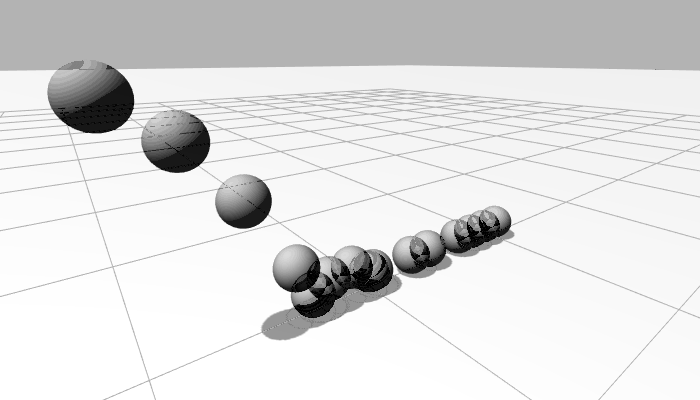
\includegraphics[width=0.8\textwidth]{images/contributions/chapter_7/bouncing_ball_trajectory.png}
    \caption{Sphere trajectory of the bouncing experiment.}
    \label{fig:bouncing_ball_trajectory}
\end{figure}

We consider a model composed of a single spherical-shaped link.
The sphere has a mass of $0.1 \, Kg$ and a radius of $10 \, cm$.
We approximate its collision shape with 500 points, all considered as collidable points for the collision detection and soft-contact model.

The sphere is positioned $1 \, m$ above a flat surface, and left falling starting from an initial linear velocity of $\vellin[B]_{W,B} = (2, 0, -1) \, m/s$.
We simulate this setting for $1.5 \, s$ using the \ac{RK4} integration scheme with a step size of $100 \, \mu s$.
The sphere's trajectory is illustrated in Figure~\ref{fig:bouncing_ball_trajectory}.

At each time instant, we compute the system's mechanical energy by summing the potential and the kinetic energies obtained from Equation~\eqref{eq:kinetic_and_potential_energies}.
We also get the linear contact forces $\forcelin[C_1]_1, \, \forcelin[C_2]_2, \, \dots$ computed with the soft-contact model of each collidable point, and combine them together in the frame $B$ of the spherical link as $\forcesix[B]_{tot} = \sum_i \transfor[B]^{C_i} \left[ \forcelin[C_i]_i^\top \;\; \zeros_3^\top \right]^\top \in \realn^6$.

Figure~\ref{fig:bouncing_ball} reports the height of the sphere corresponding to the $z$ component of $\pos[W]_B$, the plot of the mechanical energy, and the plot norm of the contact force's linear component.
It can be noticed that during the flight phase, the mechanical energy remains constant.
It gets dissipated abruptly through the contact damping upon bouncing collisions, and linearly through the terrain friction when bouncing finishes and the sphere starts rolling (corresponding to the flat region in Figure~\ref{fig:bouncing_ball_base_height}).
From the detailed view of the first two impacts reported in Figure~\ref{fig:bouncing_ball_detail1} and Figure~\ref{fig:bouncing_ball_detail2}, it can be noticed that the abrupt energy drop actually varies continuously.
From the same images, it can be seen that the soft-contact model produces contact forces that do not present marked discontinuities.
However, if the step size of the simulation becomes larger, we observed that the initial penetration depth could generate a big initial reaction force that depends on the stiffness of the terrain.
Possible solutions to mitigate this effect consists of either tuning the terrain parameters or adopting integration schemes with \emph{zero-crossing} logic that allow obtaining small initial penetration depths by shortening the integration step of the instant when the contact is made.

\begin{figure}
    \centering
    \subfloat[]{
        \includegraphics[width=0.95\textwidth]{images/contributions/chapter_7/bouncing_energy_force.tikz}
        \label{fig:bouncing_ball_complete}
    }
    \\
    \subfloat[]{
        \includegraphics[width=0.48\textwidth]{images/contributions/chapter_7/bouncing_energy_force_detail_1.tikz}
        \label{fig:bouncing_ball_detail1}
    }
    \subfloat[]{
        \includegraphics[width=0.42\textwidth]{images/contributions/chapter_7/bouncing_energy_force_detail_2.tikz}
        \label{fig:bouncing_ball_detail2}
    }
    \\
    \subfloat[]{
        \includegraphics[width=0.86\textwidth]{images/contributions/chapter_7/bouncing_base_height.tikz}
        \label{fig:bouncing_ball_base_height}
    }
    \caption{Evolution over time of the bouncing ball experiment's data. (\ref{fig:bouncing_ball_complete}) reports the mechanical energy of the system and the norm of the linear component of the contact forces summed and expressed in the $B$ frame of the spherical link. (\ref{fig:bouncing_ball_detail1}) and (\ref{fig:bouncing_ball_detail1}) report a closer view of the first two impacts. (\ref{fig:bouncing_ball_base_height}) reports the plot of the base height, where both the bouncing and rolling phases can be observed.}
    \label{fig:bouncing_ball}
\end{figure}

\subsection{Sliding Box}

We consider a model composed of a single box-shaped link.
The box has a mass of $1 \, Kg$ and $(x, y, z)$ dimensions equal to $(1.5, 1, 0.5) \, m$.
Its collision shape is approximated considering the 8 points corresponding to its corners.

The box is positioned on a flat ground surface at rest.
We simulate this setting for $4 \, s$ using the \ac{RK4} integration scheme with a step size of $1 \, ms$.
In this window, considering the frame of \ac{CoM} $G = (\pos[W]_{CoM}, [B])$, we apply to the \ac{CoM} of the box an external linear force $\forcelin[G]_{CoM} = (f_{CoM}, 0, 0) \in \realn^3$ with a profile reported in Figure~\ref{fig:sliding_box}.
The simulation is configured with a standard gravity of $g = 9.8 \, m/s$.

In this setting, the threshold of the friction cone separating the sticking and the slipping regimes is $\mu f_\perp = 4.9 \, N$, averaged over the four contacts points of the bottom box surface.
Figure~\ref{fig:sliding_box} reports the plots of the $x$ components of the \ac{CoM} position and linear velocity.
It can be seen that, as expected, when the applied force is smaller than the threshold, the box stays still.
As soon as the external force exceeds the threshold, the box starts accelerating.
As soon as the external force goes to zero, the frictional effects of the contact model produce a reaction force that decelerates the box with a fast transient until it reaches the sticking regime again.
Small velocity oscillations can be noticed when the external force is applied at $t=0.5 \, s$ and $t=1 \, s$, and when it is removed at $t=3.5 \, s$.
They can be explained by the modelled dynamics of the material that can generate small tangential deformations without leaving the sticking regime.

\begin{figure}
    \centering
    \resizebox{0.75\textwidth}{!}{
    \includegraphics{images/contributions/chapter_7/sliding_box.tikz}}
    \caption{Evolution over time of the sliding box experiment's data. From top to bottom, the first plot shows the $x$ component of the \ac{CoM} position, the second plot shows the $x$ component of the \ac{CoM} velocity, and the third plot shows the profile of the applied external force to the \ac{CoM} frame $G$.}
    \label{fig:sliding_box}
\end{figure}

\section{Conclusions}

In this chapter, we described how to model a floating-base multibody system interacting with a non-flat surface.
This formulation lays the fundamentals of a physics engine, capable of simulating the evolution of such systems in time.
We introduced a point-surface soft-contact model to compute the forces exchanged between points belonging to the links of the multibody system and a non-flat terrain, assuming to know its height profile at any point in space.
This assumption simplifies the collision detection process, requiring just trivial geometrical assessments.
The main benefit of our collisions and contacts modelling is the possibility of obtaining an extended state-space representation that includes both the dynamics of the multibody system and the dynamics of the contacts.
The contact-aware evolution of the system can be derived by any numerical integration scheme.
We validated the dynamical system in a simplified setting in which single bodies interact with a flat terrain, showing the continuity of the soft-contact model and the switching between the sticking and slipping regimes.
While sphere and box collisions might seem trivial examples, they often represent the typical collision shapes adopted to simulate robot's feet.
The shown results remain valid also in case of a smooth uneven terrain supported by the contact-model, where a comparable behaviour occurs in a different plane.

This setting presents different limitations, especially when compared to general-purpose simulators.
In fact, it does not detect the collision between different bodies and does not consider joint limits and other types of constraints.
To address the former, more advanced geometrical processing is necessary for detecting all ranges of collisions between points, primitive shapes, edges, surfaces, \etc
For the latter, instead, it is possible to introduce an additional phase in the simulation step that computes the generalized forces to apply to the system for enforcing those constraints.
